\documentclass{article}
\usepackage[utf8]{inputenc}
\usepackage[T1]{fontenc}
\usepackage{graphicx}
\usepackage{algorithm}
\usepackage{algpseudocode}

\usepackage{listings}
\usepackage{xcolor}
\usepackage[margin=2cm]{geometry}
\usepackage{float}

\usepackage{amssymb} %Ajoute des symboles mathématiques comme R, Z, forall, exists, etc....
\usepackage{amsmath}
\usepackage{amsthm}

\usepackage{enumitem}


\lstdefinestyle{monstyle}{
    backgroundcolor=\color{white},
    commentstyle=\color{gray},
    keywordstyle=\color{blue},
    numberstyle=\tiny\color{gray},
    basicstyle=\ttfamily\small,
    breaklines=true,
    numbers=left,
    numbersep=5pt,
    frame=single,
}
\lstset{style=monstyle}


\usepackage{soul} % IMPORTANT : POUR SURLIGNER AVEC \hl en fin de ligne 
\usepackage{xcolor}

\title{\sethlcolor{purple!30}\hl{Prise de notes Cours Unix pour révision : Environnement de travail}}
\author{Derrez Lorenzo}

\begin{document}
\maketitle

\section*{\sethlcolor{yellow}\hl{\textbf{Ordinateur}}}
\begin{itemize}
    \item Machine en couche $ \implies $ couche matérielle, couche d'application couche système d'exploitation 
    \item Consituée de : 
    \subitem processeurs : sert à executer les instructions du programme
    \subitem mémoire centrale : stock le programme en exécution 
    \subitem périphériques : ce qui permet d'échanger avec l'extérieur.
\end{itemize}


\section*{\sethlcolor{yellow}\hl{\textbf{Système d'exploitation}}}
\begin{itemize}
    \item logiciel qui fait le lien entre le matériel, les applications et les utilisateurs. 
    \item \textbf{SE mono-processus, mono-utilisateur} : exécute un programme à la fois avec un seul utilisateur.
    \item \textbf{SE multi-processus, mono-utilisateur} : plusieurs tâches simultanées correspondant à des programmes différents. Répartition des ressources à tour de rôle entre les applications.
    \item \textbf{SE multi-processus, multi-utilisateurs} : Plusieurs utilisateurs peuvent lancer en même temps leurs programmes sur la même machine.
\end{itemize}


\section*{\sethlcolor{yellow}\hl{\textbf{Organisation générale}}}

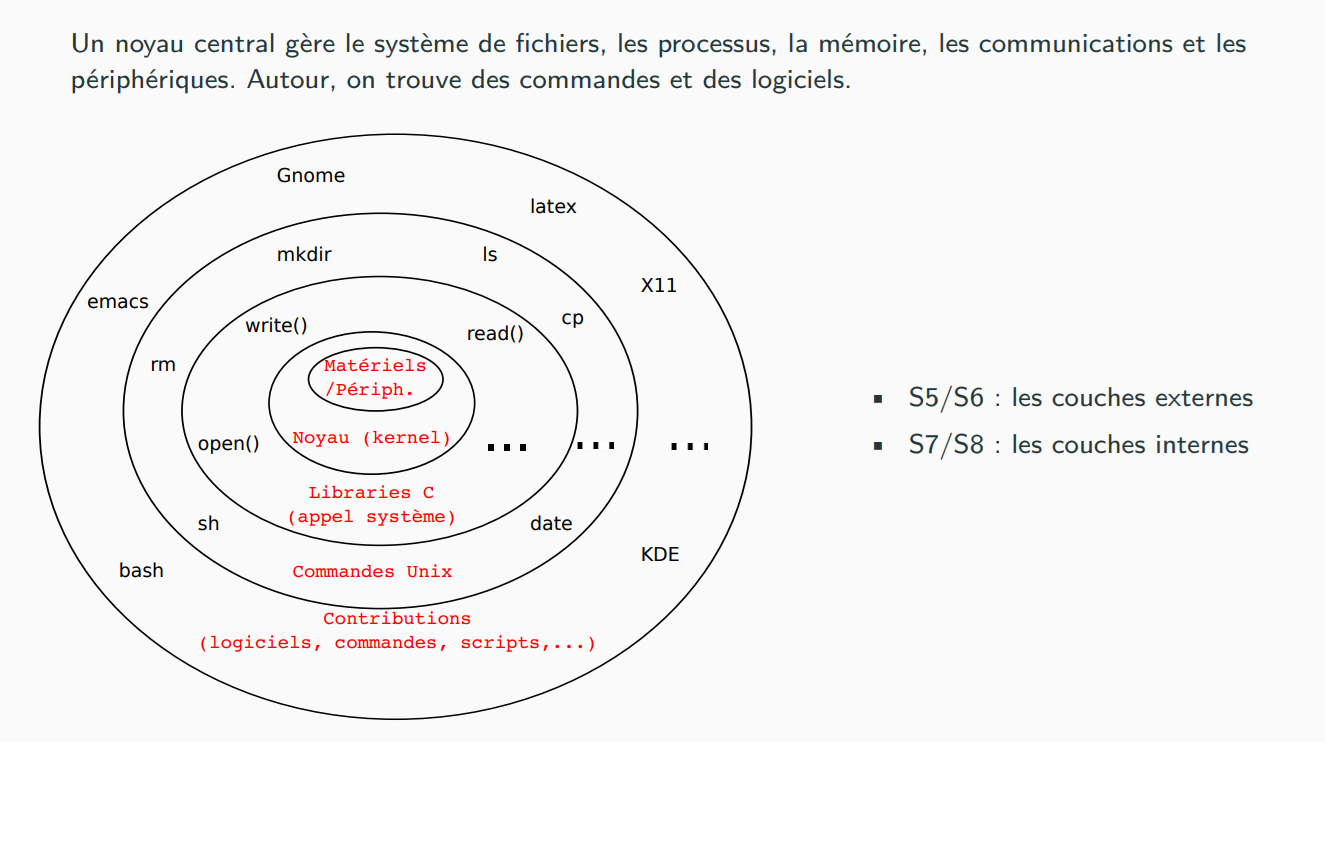
\includegraphics[width=0.70\textwidth]{schema_rev_unix.png}

\section*{\sethlcolor{yellow}\hl{Compte utilisateur \& protection}}

\begin{itemize}
    \item Système multi-processus $ \implies $ création d'un compte
    \item \textbf{Remarque :} Être responsable sur la gestion de ses mots de passe.
\end{itemize}

\section*{\sethlcolor{yellow}\hl{A propos du Shell}}

\begin{itemize}
    \item \sethlcolor{orange!30}\hl{\textbf{Shell}} : intepréteur de commande pour interagir avec le noyau.
    \item \sethlcolor{orange!30}\hl{\textbf{interpréteur de commande}} : fournit une interface texte entre l'utilisateur et le noyau.
    \item \sethlcolor{orange!30}\hl{\textbf{bash}} : programme shell par défaut dans la plupart des environnements. 
\end{itemize}

\section*{\sethlcolor{yellow}\hl{\textbf{Commandes Unix}}}

\textbf{REMARQUE} : cette liste sera ajoutée au fur et à mesures des révisions :

\begin{enumerate}[label=(\alph*)]
    \item Obtenir de l'aide pour une commande : 
    \subitem \sethlcolor{pink!30}\hl{man} nom\_de\_la\_commande
    \item Enter dans le sous-dossier \textit{divers} du sous-dossier \textit{autres} : 
    \subitem \sethlcolor{pink!30}\hl{cd} autres/divers
    \item Savoir dans quel dossier on se trouve : 
    \subitem \sethlcolor{pink!30}\hl{pwd}
    \item Lister le contenu du dossier courant : 
    \subitem \sethlcolor{pink!30}\hl{ls}
    \subitem ls -la permet d'afficher plus de détails sur le contenu
    \item Créer un répertoire : 
    \subitem \sethlcolor{pink!30}\hl{mkdir}
    \item Créer un fichier : 
    \subitem \sethlcolor{pink!30}\hl{touch}
    \item Copier (fichier ou dossier) : 
    \subitem \sethlcolor{pink!30}\hl{cp, cp-r}
    \item Déplacer/Renommer : 
    \subitem \sethlcolor{pink!30}\hl{mv}
    \item Déterminer le type d'un contenu : 
    \subitem \sethlcolor{pink!30}\hl{file}
    \item Afficher un fichier : 
    \subitem \sethlcolor{pink!30}\hl{cat}
    \item Parcourir un fichier : 
    \subitem \sethlcolor{pink!30}\hl{less}
    \item Compter (ligne, lettre, mot, etc...) : 
    \subitem \sethlcolor{pink!30}\hl{wc, wc -l, wc -w}
    \item Supprimer un contenu : 
    \subitem \sethlcolor{pink!30}\hl{rm}
    \item Modifier les droits : 
    \subitem \sethlcolor{pink!30}\hl{chmod}
\end{enumerate}

\section*{\sethlcolor{yellow}\hl{\textbf{A propos des droits de fichiers :}}}

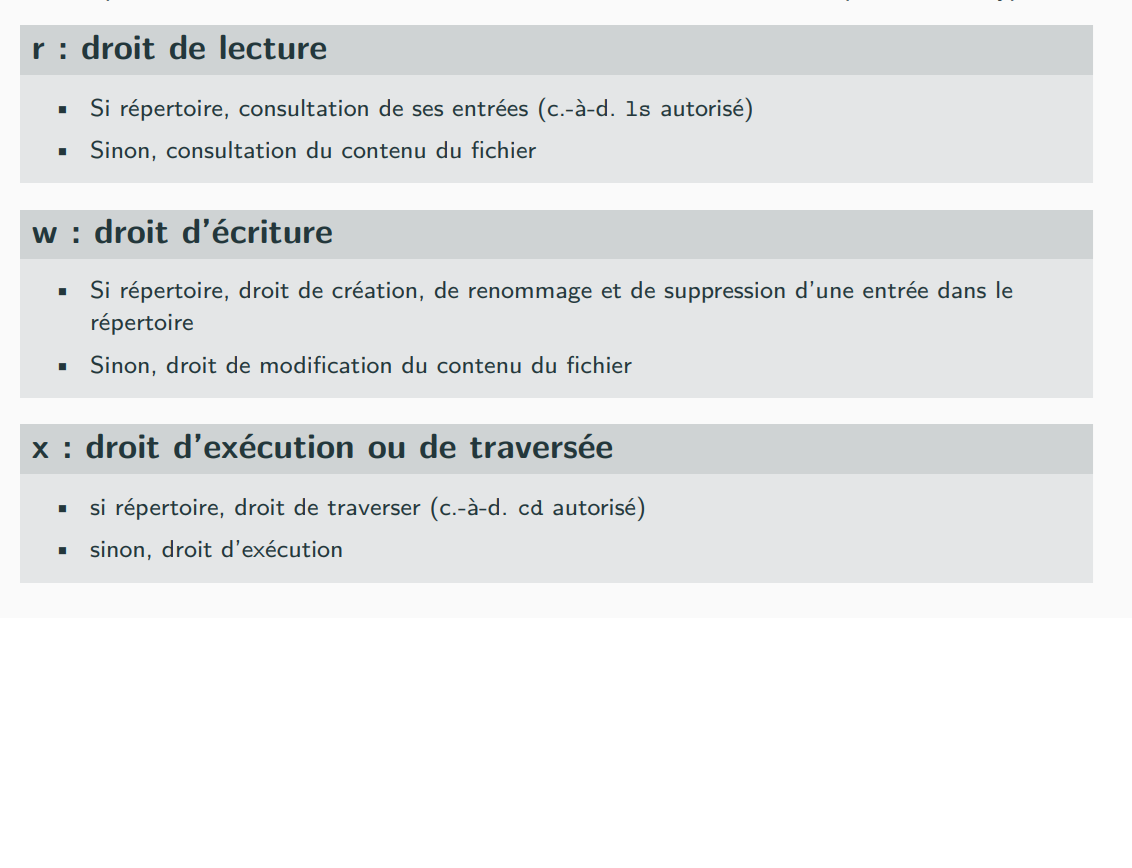
\includegraphics[width=0.70\textwidth]{droit_fichier.png}

\hl{\textbf{3 catégories d'utilisateurs :}}
\begin{itemize}
    \item Propriétaires (u : user)
    \item Groupe propriétaire (g : group)
    \item Tous les autres (o : other)
\end{itemize}

\textbf{Pour l'affichage}, on a à la suite :
\begin{itemize}
    \item - $ \implies$ Type de fichier
    \item - - - $ \implies $ Droits du propriétaire (rwx)
    \item - - - $ \implies $ Droits du groupe (rwx)
    \item - - - $ \implies $ Droits des autres (rwx)
\end{itemize}

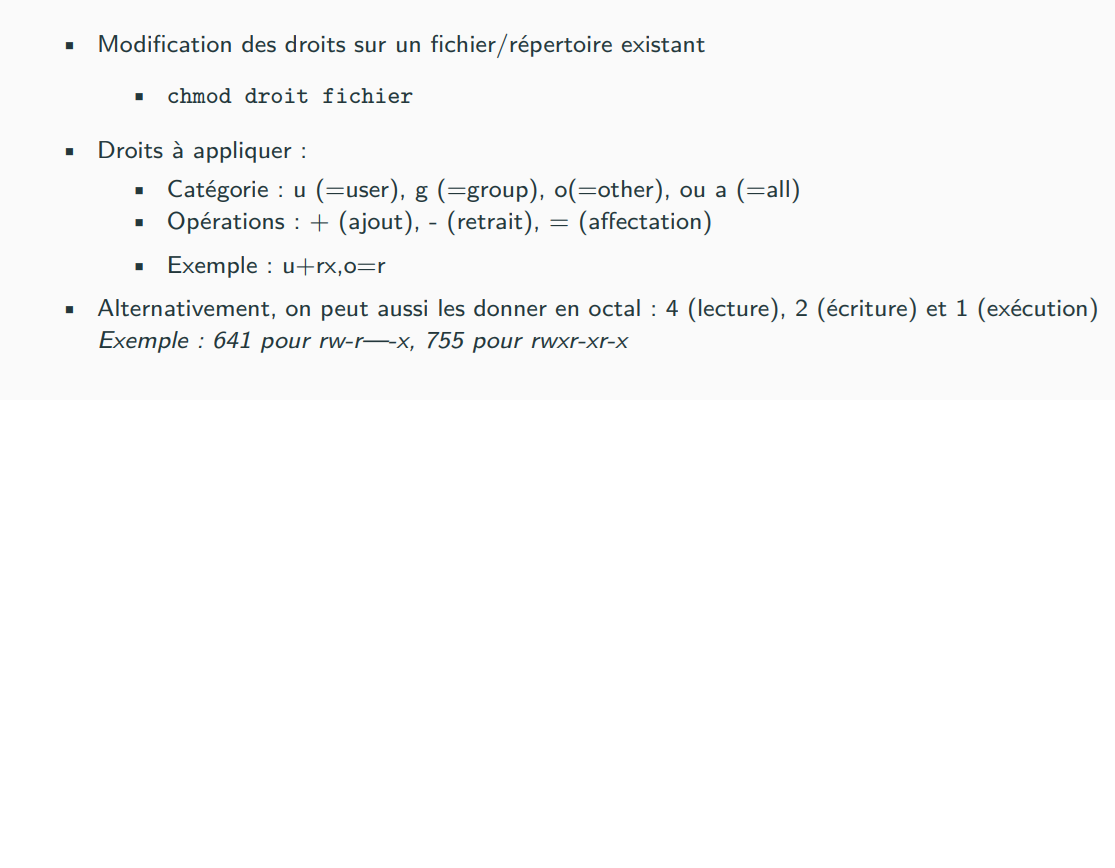
\includegraphics[width=0.70\textwidth]{modif_droits.png}

\section*{\sethlcolor{yellow}\hl{Raccourcis Shell}}

\begin{enumerate}[label=(\alph*)]
    \item Recherche avec motif : \sethlcolor{pink!30}\hl{C-r}
    \item Commande précédente : \sethlcolor{pink!30}\hl{C-p}
    \item Commande suivante : \sethlcolor{pink!30}\hl{C-n}
    \item Historique des commandes : \sethlcolor{pink!30}\hl{history}
    \item Couper/mémoriser le texte depuis la position du curseur jusqu'à la fin de la ligne : \sethlcolor{pink!30}\hl{C-k}
    \item Insérer le texte précédent supprimé : \sethlcolor{pink!30}\hl{C-y}
    \item Début de ligne : \sethlcolor{pink!30}\hl{C-a}
    \item Fin de ligne : \sethlcolor{pink!30}\hl{C-e}
    \item Activer la complétion : \sethlcolor{pink!30}\hl{tab}
    \item Pour contrôler le processus courant : 
    \subitem Lancer en tâche de fond : \sethlcolor{pink!30}\hl{cmd \&}
    \subitem Endormir le processus en cours : \sethlcolor{pink!30}\hl{C-z}
    \subitem terminer le processus en cours : \sethlcolor{pink!30}\hl{C-c}
    \subitem Quitter le shell en cours : \sethlcolor{pink!30}\hl{C-d}
    \item Pour manipuler les jobs du shell : 
    \subitem Lister les jobs connus du shell : \sethlcolor{pink!30}\hl{jobs}
    \subitem Réveiller un job en tâche de fond : \sethlcolor{pink!30}\hl{bg n}
    \subitem Remettre un job au premier plan : \sethlcolor{pink!30}\hl{fg n}
    \item Obtenir la liste des processus : \sethlcolor{pink!30}\hl{ps}
    \item Obtenit le PID de la dernière commande lancée en tâche de fond : \sethlcolor{pink!30}\hl{echo \&}
    \item Demander l'arrêt d'un processus spécifique : \sethlcolor{pink!30}\hl{kill pid}
    \item Forcer l'arrêt d'un processus spécifique : \sethlcolor{pink!30}\hl{kill -KILL pid}
\end{enumerate}

\section*{\sethlcolor{yellow}\hl{Arborescence et système de fichiers}}

\begin{itemize}
    \item Les fichiers sont structurés sous la forme d'un arbre. 
    \item Noeuds $ \implies $ répertoire.
    \item Feuilles $ \implies $ fichiers réguliers. 
\end{itemize}

\sethlcolor{pink!30}\hl{\textbf{Arborescence standard :}}
\\
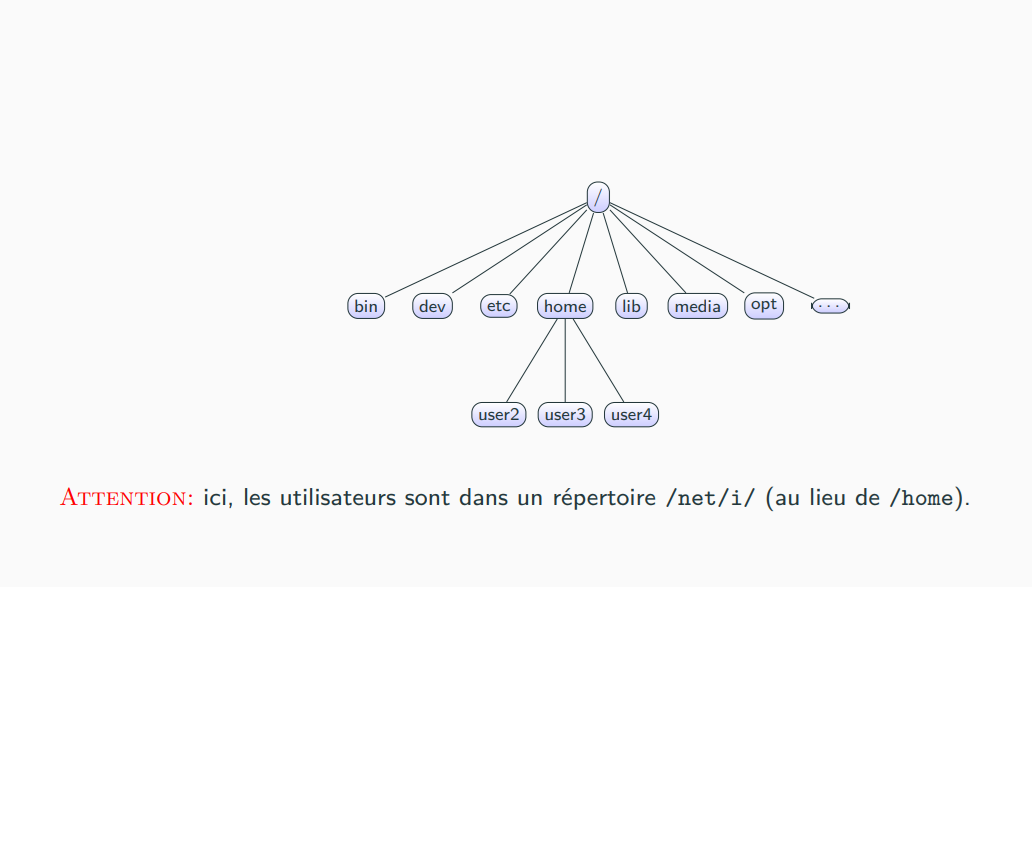
\includegraphics[width=0.70\textwidth]{arbo_standard.png}

\sethlcolor{pink!30}\hl{\textbf{Chemins absolus :}}
\\
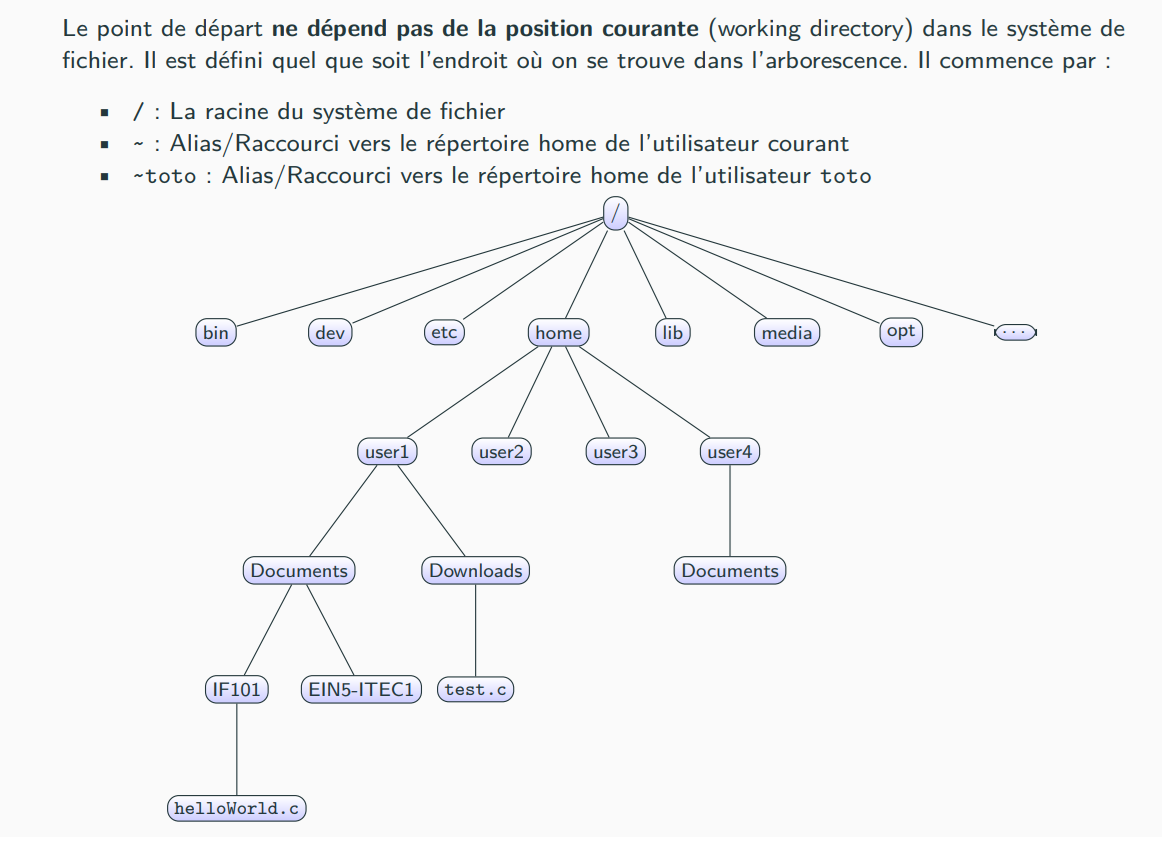
\includegraphics[width=0.70\textwidth]{chemin_absolus.png}

\sethlcolor{pink!30}\hl{\textbf{Chemins relatifs :}}
\\
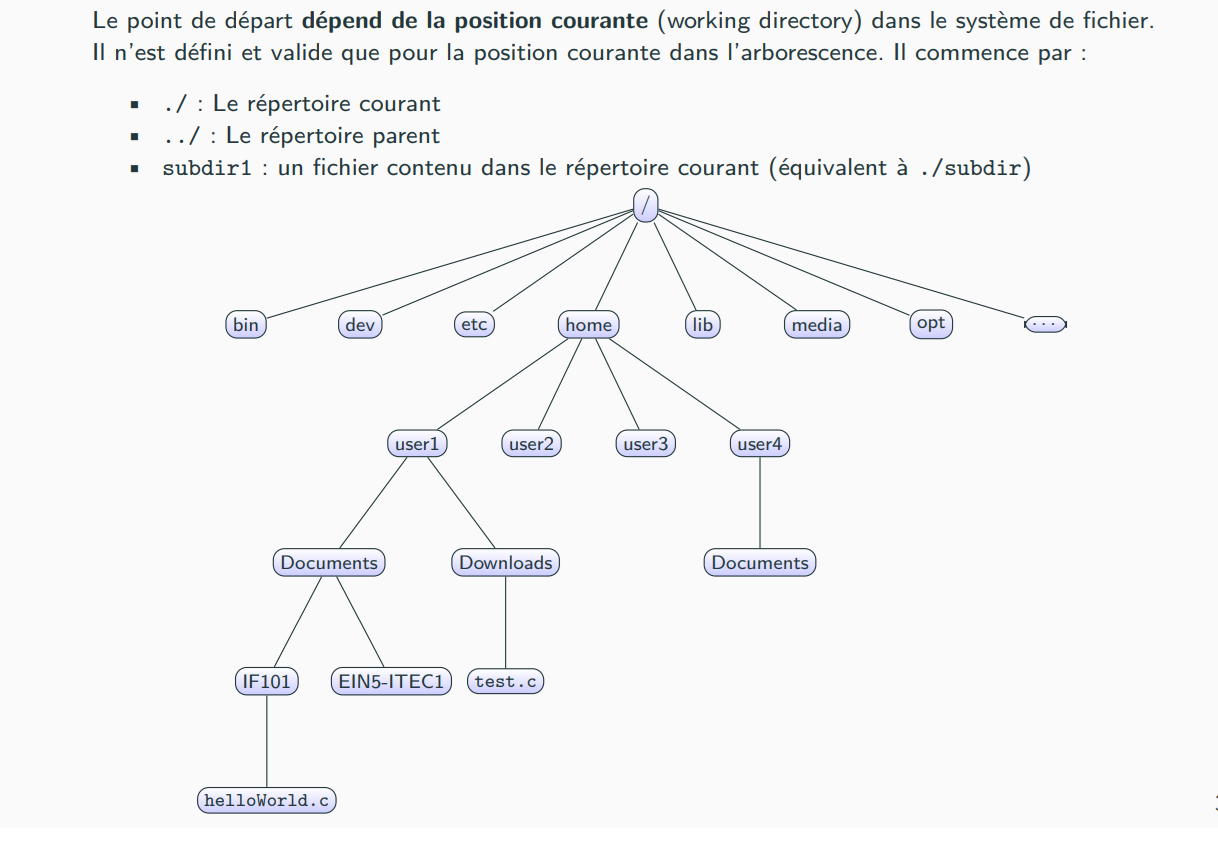
\includegraphics[width=0.70\textwidth]{chemin_relatifs.png}

\section*{\sethlcolor{yellow}\hl{\textbf{Substitutions et variables}}}

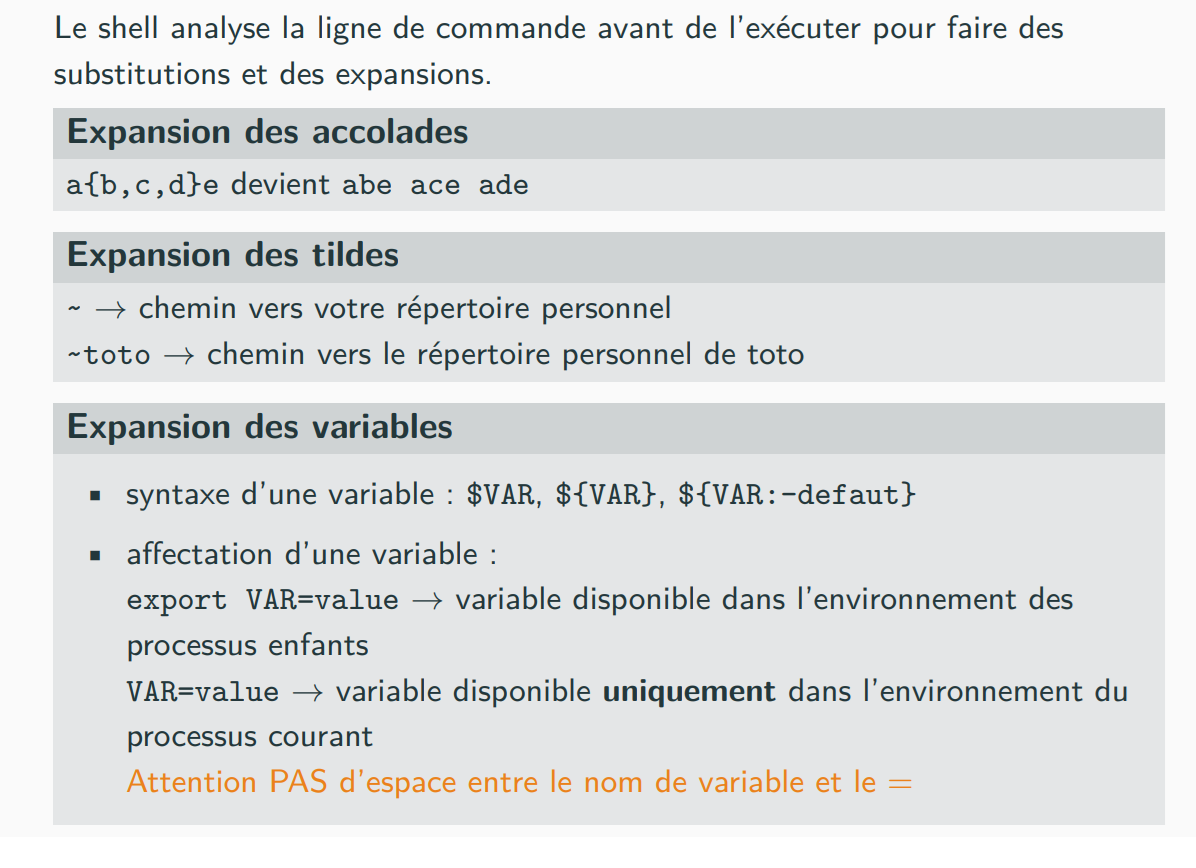
\includegraphics[width=0.70\textwidth]{substi1.png}
\\
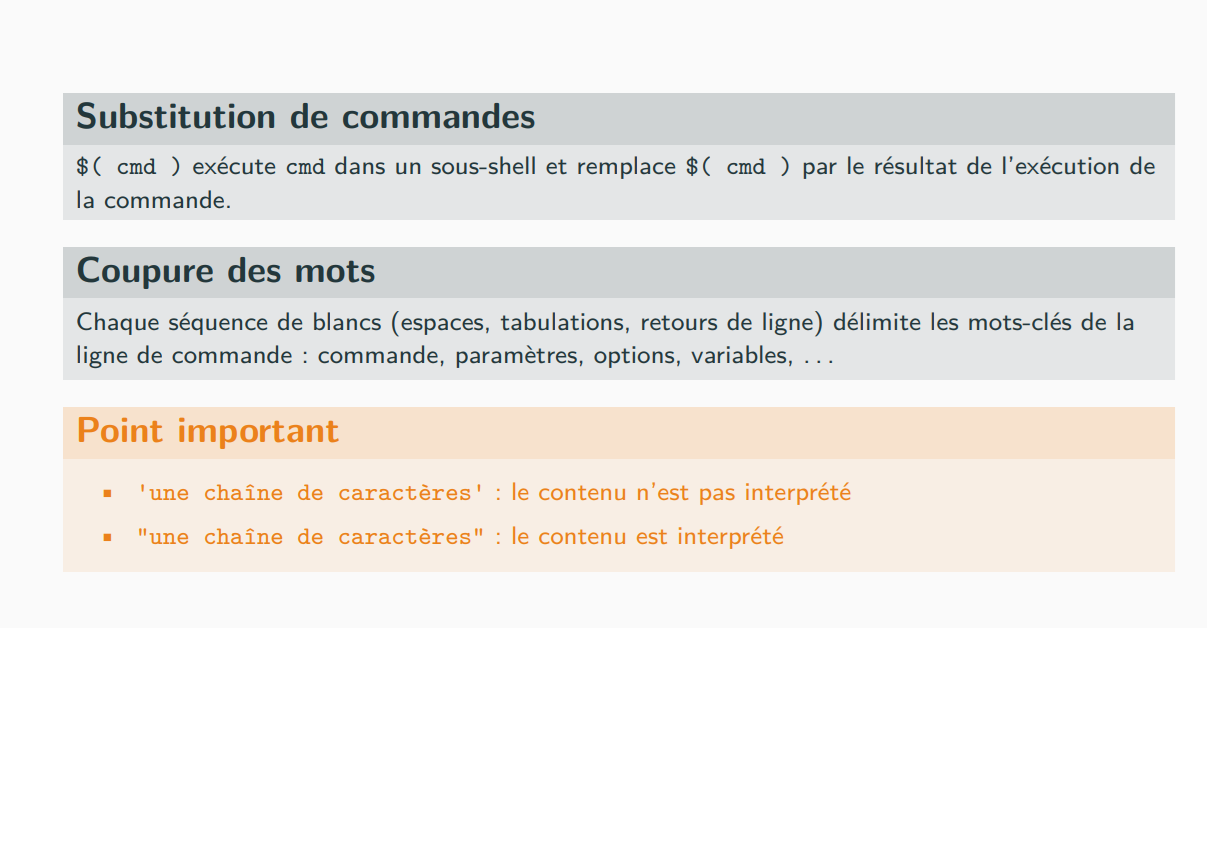
\includegraphics[width=0.70\textwidth]{substi2.png}
\\
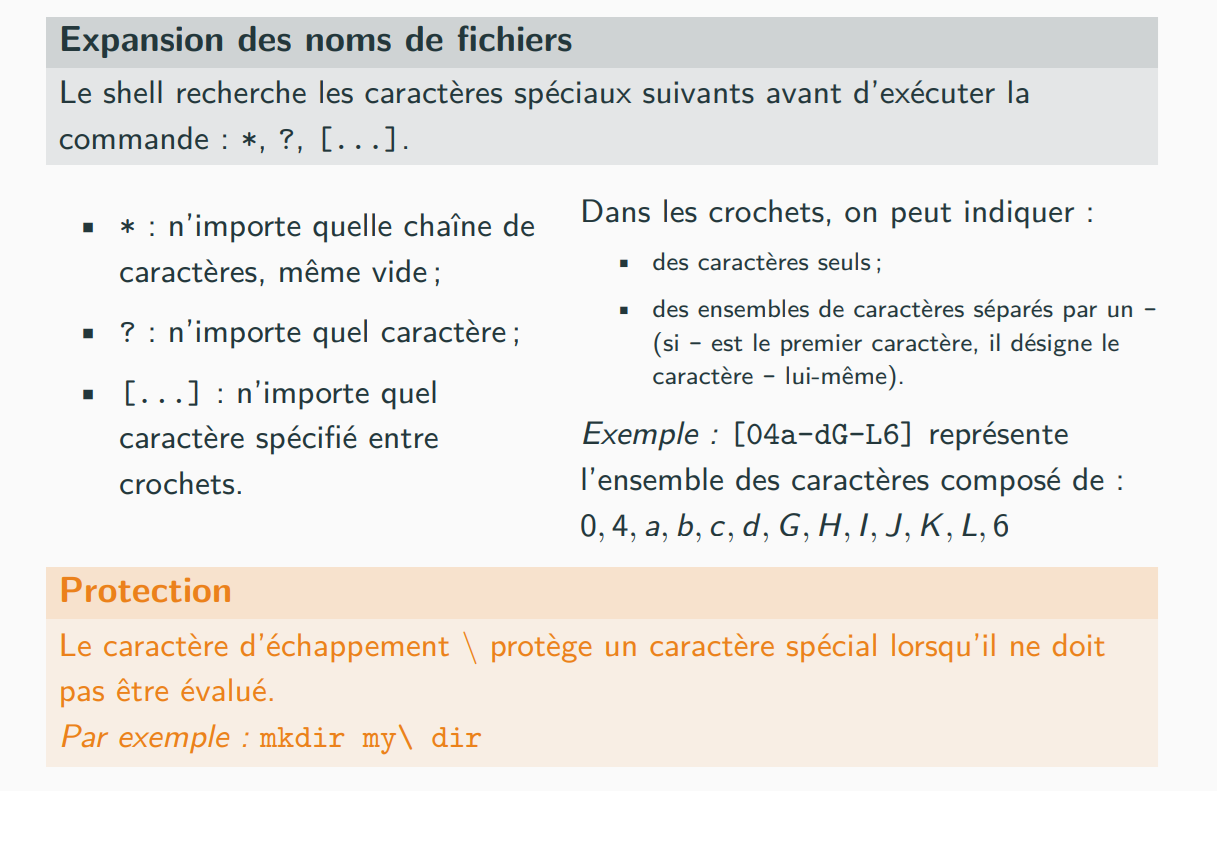
\includegraphics[width=0.70\textwidth]{substi3.png}

\section*{\sethlcolor{yellow}\hl{\textbf{Mécanismes d'entrées/sorties}}}

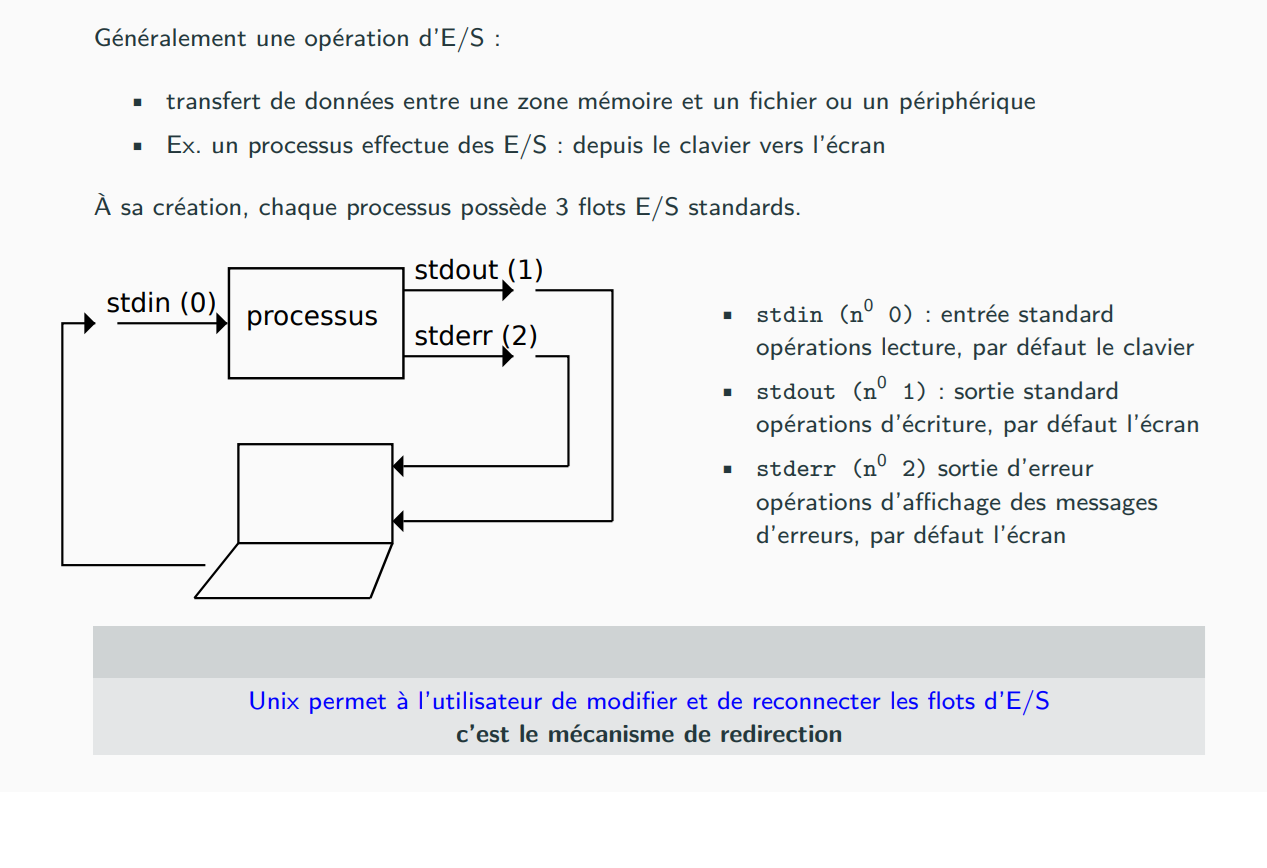
\includegraphics[width=0.70\textwidth]{sche_meca_entree_sortie.png}
\\
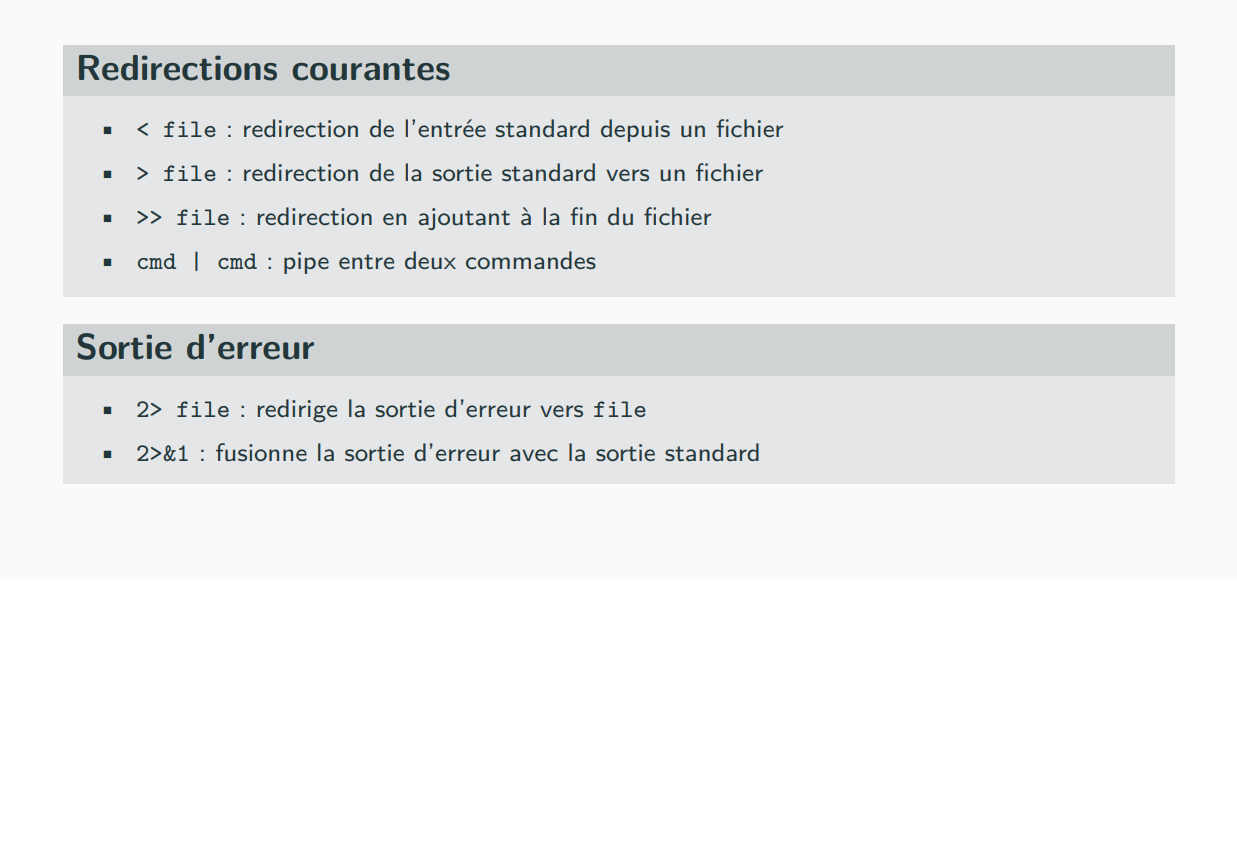
\includegraphics[width=0.70\textwidth]{meca_entree_sorties.png}

\end{document}